\documentclass[14pt]{extbook}
\usepackage{multicol, enumerate, enumitem, hyperref, color, soul, setspace, parskip, fancyhdr} %General Packages
\usepackage{amssymb, amsthm, amsmath, bbm, latexsym, units, mathtools} %Math Packages
\everymath{\displaystyle} %All math in Display Style
% Packages with additional options
\usepackage[headsep=0.5cm,headheight=12pt, left=1 in,right= 1 in,top= 1 in,bottom= 1 in]{geometry}
\usepackage[usenames,dvipsnames]{xcolor}
\usepackage{dashrule}  % Package to use the command below to create lines between items
\newcommand{\litem}[1]{\item#1\hspace*{-1cm}\rule{\textwidth}{0.4pt}}
\pagestyle{fancy}
\lhead{Makeup Progress Quiz 3}
\chead{}
\rhead{Version A}
\lfoot{4315-3397}
\cfoot{}
\rfoot{Fall 2020}
\begin{document}

\begin{enumerate}
\litem{
Solve the rational equation below. Then, choose the interval(s) that the solution(s) belongs to.\[ \frac{49}{14x -21} + 1 = \frac{49}{14x -21} \]\begin{enumerate}[label=\Alph*.]
\item \( x_1 \in [-0.5, 2.5] \text{ and } x_2 \in [0.5,3.5] \)
\item \( x \in [-1.5,0.5] \)
\item \( \text{All solutions lead to invalid or complex values in the equation.} \)
\item \( x_1 \in [-1.5, 0.5] \text{ and } x_2 \in [0.5,3.5] \)
\item \( x \in [1.5,3.5] \)

\end{enumerate} }
\litem{
Solve the rational equation below. Then, choose the interval(s) that the solution(s) belongs to.\[ \frac{-2x}{-2x + 5} + \frac{-5x^{2}}{10x^{2} -33 x + 20} = \frac{3}{-5x + 4} \]\begin{enumerate}[label=\Alph*.]
\item \( x_1 \in [-2.05, 0] \text{ and } x_2 \in [2.22,3] \)
\item \( \text{All solutions lead to invalid or complex values in the equation.} \)
\item \( x \in [0.59,1.07] \)
\item \( x_1 \in [-2.05, 0] \text{ and } x_2 \in [1.45,2.18] \)
\item \( x \in [1.54,2.42] \)

\end{enumerate} }
\litem{
Choose the graph of the equation below.\[ f(x) = \frac{-1}{(x + 3)^2} - 2 \]\begin{enumerate}[label=\Alph*.]
\begin{multicols}{2}\item 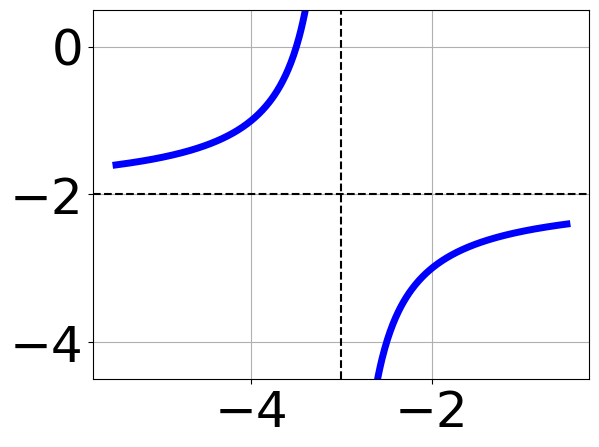
\includegraphics[width = 0.3\textwidth]{../Figures/rationalEquationToGraphCopyAA.png}\item 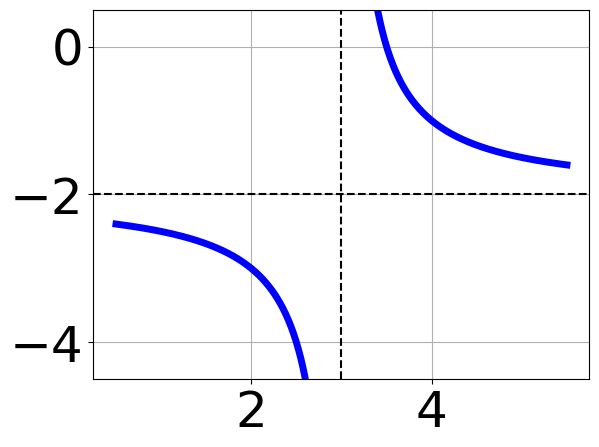
\includegraphics[width = 0.3\textwidth]{../Figures/rationalEquationToGraphCopyBA.png}\item 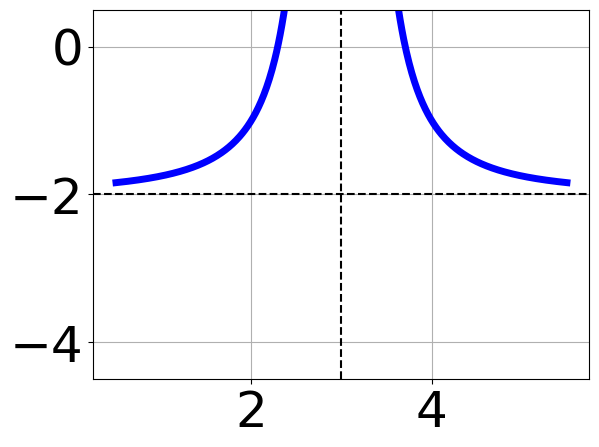
\includegraphics[width = 0.3\textwidth]{../Figures/rationalEquationToGraphCopyCA.png}\item 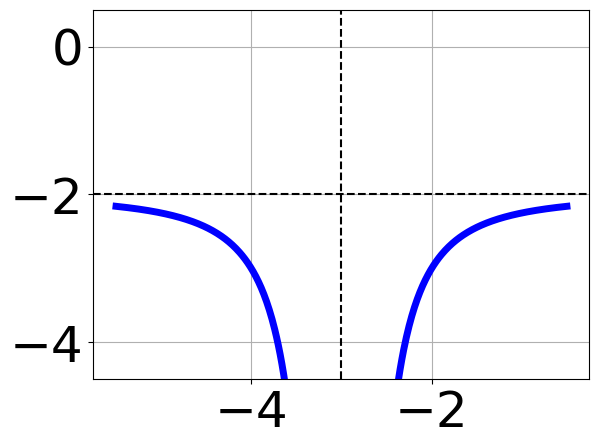
\includegraphics[width = 0.3\textwidth]{../Figures/rationalEquationToGraphCopyDA.png}\end{multicols}\item None of the above.
\end{enumerate} }
\litem{
Determine the domain of the function below.\[ f(x) = \frac{6}{16x^{2} -4 x -30} \]\begin{enumerate}[label=\Alph*.]
\item \( \text{All Real numbers except } x = a \text{ and } x = b, \text{ where } a \in [-1.4, -1.1] \text{ and } b \in [-0.7, 2] \)
\item \( \text{All Real numbers except } x = a, \text{ where } a \in [-1.4, -1.1] \)
\item \( \text{All Real numbers.} \)
\item \( \text{All Real numbers except } x = a, \text{ where } a \in [-20.5, -17.7] \)
\item \( \text{All Real numbers except } x = a \text{ and } x = b, \text{ where } a \in [-20.5, -17.7] \text{ and } b \in [23.2, 24.2] \)

\end{enumerate} }
\litem{
Choose the equation of the function graphed below.
\begin{center}
    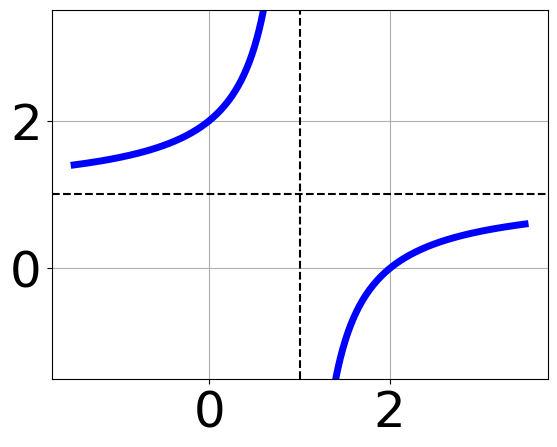
\includegraphics[width=0.5\textwidth]{../Figures/rationalGraphToEquationA.png}
\end{center}
\begin{enumerate}[label=\Alph*.]
\item \( f(x) = \frac{-1}{(x + 1)^2} + 1 \)
\item \( f(x) = \frac{1}{x - 1} + 1 \)
\item \( f(x) = \frac{1}{(x - 1)^2} + 1 \)
\item \( f(x) = \frac{-1}{x + 1} + 1 \)
\item \( \text{None of the above} \)

\end{enumerate} }
\litem{
Determine the domain of the function below.\[ f(x) = \frac{5}{20x^{2} +46 x + 24} \]\begin{enumerate}[label=\Alph*.]
\item \( \text{All Real numbers.} \)
\item \( \text{All Real numbers except } x = a, \text{ where } a \in [-24.89, -23.8] \)
\item \( \text{All Real numbers except } x = a, \text{ where } a \in [-1.91, -1.37] \)
\item \( \text{All Real numbers except } x = a \text{ and } x = b, \text{ where } a \in [-24.89, -23.8] \text{ and } b \in [-20.58, -19.95] \)
\item \( \text{All Real numbers except } x = a \text{ and } x = b, \text{ where } a \in [-1.91, -1.37] \text{ and } b \in [-1.34, -0.73] \)

\end{enumerate} }
\litem{
Solve the rational equation below. Then, choose the interval(s) that the solution(s) belongs to.\[ \frac{4x}{4x -6} + \frac{-7x^{2}}{8x^{2} -20 x + 12} = \frac{3}{2x -2} \]\begin{enumerate}[label=\Alph*.]
\item \( x_1 \in [0.89, 0.96] \text{ and } x_2 \in [-4.5,2.5] \)
\item \( x_1 \in [0.89, 0.96] \text{ and } x_2 \in [17.05,21.05] \)
\item \( x \in [19.04,19.06] \)
\item \( \text{All solutions lead to invalid or complex values in the equation.} \)
\item \( x \in [0.95,1.01] \)

\end{enumerate} }
\litem{
Solve the rational equation below. Then, choose the interval(s) that the solution(s) belongs to.\[ \frac{-8}{3x -9} + 9 = \frac{9}{15x -45} \]\begin{enumerate}[label=\Alph*.]
\item \( x \in [-3.64,-0.64] \)
\item \( x \in [2.36,5.36] \)
\item \( x_1 \in [-3.64, -0.64] \text{ and } x_2 \in [1.9,3.5] \)
\item \( x_1 \in [2.36, 6.36] \text{ and } x_2 \in [3.4,3.8] \)
\item \( \text{All solutions lead to invalid or complex values in the equation.} \)

\end{enumerate} }
\litem{
Choose the equation of the function graphed below.
\begin{center}
    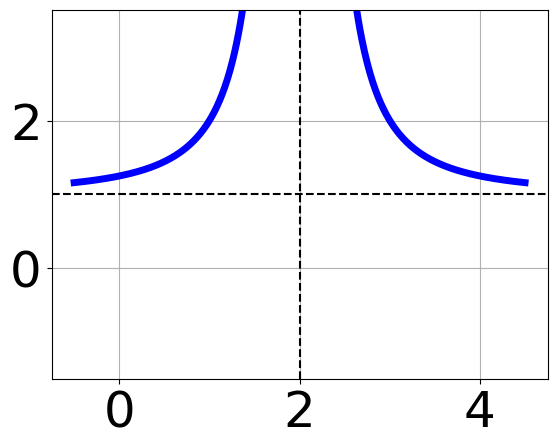
\includegraphics[width=0.5\textwidth]{../Figures/rationalGraphToEquationCopyA.png}
\end{center}
\begin{enumerate}[label=\Alph*.]
\item \( f(x) = \frac{-1}{x + 2} - 4 \)
\item \( f(x) = \frac{1}{(x - 2)^2} - 4 \)
\item \( f(x) = \frac{-1}{(x + 2)^2} - 4 \)
\item \( f(x) = \frac{1}{x - 2} - 4 \)
\item \( \text{None of the above} \)

\end{enumerate} }
\litem{
Choose the graph of the equation below.\[ f(x) = \frac{1}{x - 3} - 2 \]\begin{enumerate}[label=\Alph*.]
\begin{multicols}{2}\item 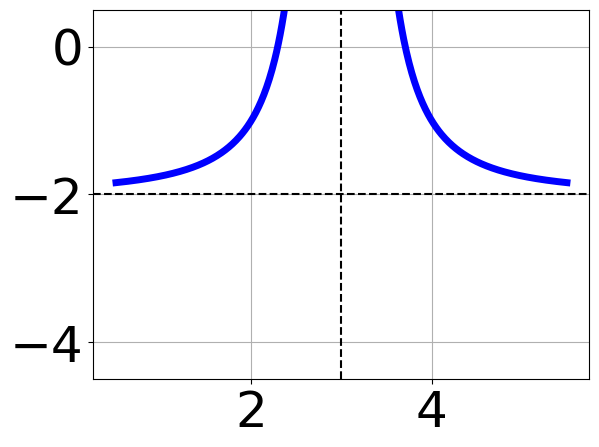
\includegraphics[width = 0.3\textwidth]{../Figures/rationalEquationToGraphAA.png}\item 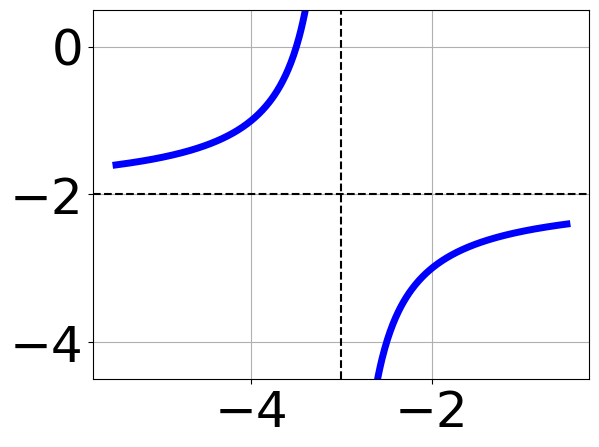
\includegraphics[width = 0.3\textwidth]{../Figures/rationalEquationToGraphBA.png}\item 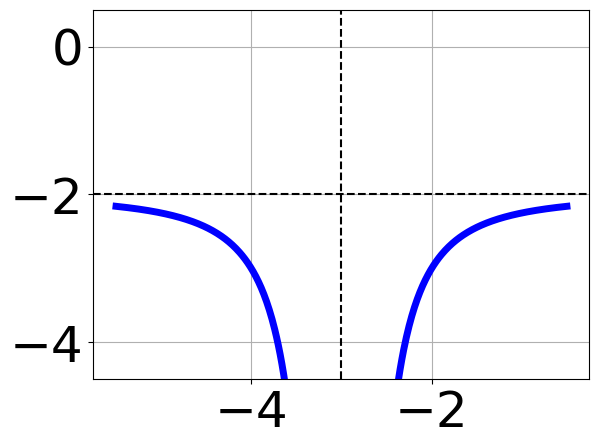
\includegraphics[width = 0.3\textwidth]{../Figures/rationalEquationToGraphCA.png}\item 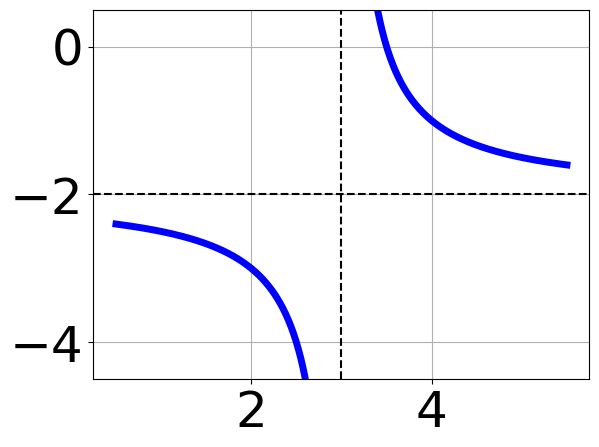
\includegraphics[width = 0.3\textwidth]{../Figures/rationalEquationToGraphDA.png}\end{multicols}\item None of the above.
\end{enumerate} }
\end{enumerate}

\end{document}